 \documentclass [12pt]{article} 

\usepackage {amsmath}
\usepackage {amsthm}
\usepackage {amssymb}
\usepackage {graphicx} 
\usepackage {float}
\usepackage {multirow}
\usepackage {xcolor}
\usepackage {algorithmic}
\usepackage [ruled,vlined,commentsnumbered,titlenotnumbered]{algorithm2e} \usepackage {array} 
\usepackage {booktabs} 
\usepackage {url} 
\usepackage {parskip} 
\usepackage [margin=1in]{geometry} 
\usepackage [T1]{fontenc} 
\usepackage {cmbright} 
\usepackage [many]{tcolorbox} 
\usepackage [colorlinks = true,
            linkcolor = blue,
            urlcolor  = blue,
            citecolor = blue,
            anchorcolor = blue]{hyperref} 
\usepackage {enumitem} 
\usepackage {xparse} 
\usepackage {verbatim}
\usepackage{listings}
\usepackage{xcolor}
\lstset { %
    language=C++,
    backgroundcolor=\color{black!5}, % set backgroundcolor
    basicstyle=\footnotesize,% basic font setting
}
\newtheorem{theorem}{Theorem}
\newtheorem{remark}{Remark}



\DeclareTColorBox {Solution}{}{breakable, title={Solution}} \DeclareTColorBox {Solution*}{}{breakable, title={Solution (provided)}} \DeclareTColorBox {Instruction}{}{boxrule=0pt, boxsep=0pt, left=0.5em, right=0.5em, top=0.5em, bottom=0.5em, arc=0pt, toprule=1pt, bottomrule=1pt} \DeclareDocumentCommand {\Expecting }{+m}{\textbf {[We are expecting:} #1\textbf {]}} \DeclareDocumentCommand {\Points }{m}{\textbf {(#1 pt.)}} 

\begin {document} 

\vspace {1em} 
\begin {Instruction} 
Adapted From Virginia Williams' lecture notes.
\end {Instruction}  

{\LARGE \textbf {COMP 285 (NC A\&T, Spr `22)}\hfill \textbf {Lecture 15} } 

\begin{centering}
\section*{Graphs and Depth-First Search}
\end{centering}

\section{Graphs}
A graph is a set of vertices and edges connecting those vertices. Formally, we define a graph $G$ as $G = (V, E)$ where $E \subseteq V \times V$ . For ease of analysis, the variables $n$ and $m$ typically stand for the number of vertices and edges, respectively. Graphs can come in two flavors, directed or undirected. If a graph is undirected, it must satisfy the property that $(i, j) \in E \iff (j, i) \in E$ (i.e., all edges are bidirectional). In undirected graphs, $m \leq \frac{n(n-1)}{2}$ . In directed graphs, $m \leq n(n - 1)$. Thus, $m = O(n^2)$ and $\log m = O(\log n)$. A connected graph is a graph in which for any two nodes $u$ and $v$ there exists a path from $u$ to $v$ . For an undirected connected graph $m \geq n - 1$. A sparse graph is a graph with few edges (for example, $\Theta(n)$ edges) while a dense graph is a graph with many edges (for example, $m = \Theta(n^2)$).

\subsection{Representation} 

A common issue is the topic of how to represent a graph's edges in memory. There are two standard methods for this task. 

An \textbf{adjacency matrix} uses an arbitrary ordering of the vertices from $1$ to $|V|$. The matrix consists of an $n \times n$ binary matrix such that the $(i, j)$-th element is $1$ if $(i, j)$ is an edge in the graph, $0$ otherwise. 

An \textbf{adjacency list} consists of an array $A$ of $|V |$ lists, such that $$A[u]$$ contains a linked list of vertices $v$ such that $(u, v) \in E$ (the neighbors of $u$). In the case of a directed graph, it's also helpful to distinguish between outgoing and ingoing edges by storing two different lists at $A[u]$: a list of $v$ such that $(u, v ) \in E$ (the out-neighbors of $u$) as well as a list of $v$ such that $(v, u) \in E$ (the in-neighbors of $u$). 

What are the tradeoffs between these two methods? To help our analysis, let deg($v$) denote the \textbf{degree} of $v$, or the number of vertices connected to $v$. In a directed graph, we can distinguish between out-degree and in-degree, which respectively count the number of outgoing and incoming edges.

\begin{itemize}
  \item The adjacency matrix can check if $(i, j)$ is an edge in $G$ in constant time, whereas the adjacency list representation must iterate through up to deg($i$) list entries.
  \item The adjacency matrix takes $\Theta(n^2)$ space, whereas the adjacency list takes $\Theta(m + n)$ space.
  \item The adjacency matrix takes $\Theta(n)$ operations to enumerate the neighbors of a vertex v since it must iterate across an entire row of the matrix. The adjacency list takes deg($v $) time.
\end{itemize}
 
What's a good rule of thumb for picking the implementation? One useful property is the sparsity of the graph's edges. If the graph is \textbf{sparse}, and the number of edges is considerably less than the max ($m \ll n^2$ ), then the adjacency list is a good idea. If the graph is dense and the number of edges is nearly $n^2$ , then the matrix representation makes sense because it speeds up lookups without too much space overhead. Of course, some applications will have lots of space to spare, making the matrix feasible no matter the structure of the graphs. Other applications may prefer adjacency lists even for dense graphs. Choosing the appropriate structure is a balancing act of requirements and priorities.

\section{Depth First Search (DFS)} 

Given a starting vertex, it's desirable to find all vertices reachable from the start. There are many algorithms to do this, the simplest of which is depth-first search. As the name implies, DFS enumerates the deepest paths, only backtracking when it hits a dead end or an already-explored section of the graph. DFS by itself is fairly simple, so we introduce some augmentations to the basic algorithm. 

\begin{itemize}
  \item To prevent loops, DFS keeps track of a ``color'' attribute for each vertex. Unvisited vertices are white by default. Vertices that have been visited but still may be backtracked to are colored gray. Vertices which are completely processed are colored black. The algorithm can then prevent loops by skipping non-white vertices
  \item Instead of just marking visited vertices, the algorithm also keeps track of the tree generated by the depth-first traversal. It does so by marking the ``parent'' of each visited vertex, aka the vertex that DFS visited immediately prior to visiting the child.
  \item The augmented DFS also marks two auto-incrementing timestamps $d$ and $f$ to indicate when a node was first discovered and finished.
\end{itemize}

The algorithm takes as input a start vertex $s$ and a starting timestamp $t$, and returns the timestamp at which the algorithm finishes. Let $N(s)$ denote the neighbors of $s$; for a directed graph, let $N_{\text{out}}(s)$ denote the out-neighbors of $s$.

\begin{algorithm}
\caption{\texttt{init}(G)}
\label{alg:init_G}
\begin{algorithmic}
\FOR {$v \in G$}
\STATE color($v$) $\gets$ white
\STATE d($v$), f($v$) $\gets \infty$ 
\STATE p($v$) $\gets$ nil
\ENDFOR
\end{algorithmic}
\end{algorithm}

\begin{algorithm}
\caption{\texttt{DFS}(s, t): $s \in V$ is white, $t =$ time}
\label{alg:DFS_s_t}
\begin{algorithmic}
\STATE color(s) $\gets$ gray
\STATE \texttt{// d(s) is the discovery time of s}
\STATE $d(s) \gets t$
\STATE $t \gets t+1$
\FOR {$v \in N(s)$}
  \IF {$color(v) = white$}
    \STATE $p(v) \gets s$
    \STATE \texttt{// Update t to be the finish time of DFS starting at v}
    \STATE $t \gets DFS(v,t)$
    \STATE $t \gets t + 1$
  \ENDIF
\ENDFOR
\STATE \texttt{Finish time:}
\STATE $f(s) \gets t$
\STATE \texttt{// s is finished}
\STATE color($s$) $\gets$ black
\end{algorithmic}
\end{algorithm}

There are multiple ways we can search using DFS. One way is to search from some source node $s$, which will give us a set of black nodes reachable from $s$ and white nodes unreachable from $s$.

\begin{algorithm}
\caption{\texttt{DFS}(s): DFS from a source node $s$}
\label{alg:DFS_s}
\begin{algorithmic}
\STATE init($G$)
\STATE DFS($s, 1$)
\end{algorithmic}
\end{algorithm}

Another way to use DFS is to search over the entire graph, choosing some white node and finding everything we can reach from that node, and repeating until we have no white nodes remaining. In an undirected graph this will give us all of the connected components.

\begin{algorithm}
\caption{\texttt{DFS}(G): DFS on an entire graph $G$}
\label{alg:DFS_G}
\begin{algorithmic}
\STATE init($G$)
\STATE $t \gets 1$
\FOR {$ v \in G$}
  \IF {$color(v) = white$}
    \STATE $t \gets$ DFS($v,t$)
    \STATE $t \gets t+1$
  \ENDIF
\ENDFOR
\end{algorithmic}
\end{algorithm}

\subsection{Runtime of DFS} 

We will now look at the runtime for the standard DFS algorithm (\ref{alg:DFS_s_t}). 

Everything above the loop runs in $O(1)$ time per node visit. Excluding the recursive call, everything inside of the for loop takes $O(1)$ time every time an edge is scanned. Everything after the for loop also runs in $O(1)$ time per node visit. 

We can express the runtime of DFS as $O(\#\text{ of node visits }+ \# \text{ of edge scans})$. Assume we have a graph with $n$ nodes and $m$ edges. We know that the \# of node visits is $\leq n$, since we only visit white nodes and whenever we visit a node we change its color from white to gray and never change it back to white again. We also know that an edge $(u, v)$ is scanned only when $u$ or $v$ is visited. Since every node is visited at most once, we know that an edge $(u, v)$ is scanned at most twice (or only once for directed graphs). Thus, \# of edges scanned is $O(m)$, and the overall runtime of DFS is $O(m + n)$.

\subsection{DFS Example}
We will now try running DFS on the example graph below.
\begin{center}
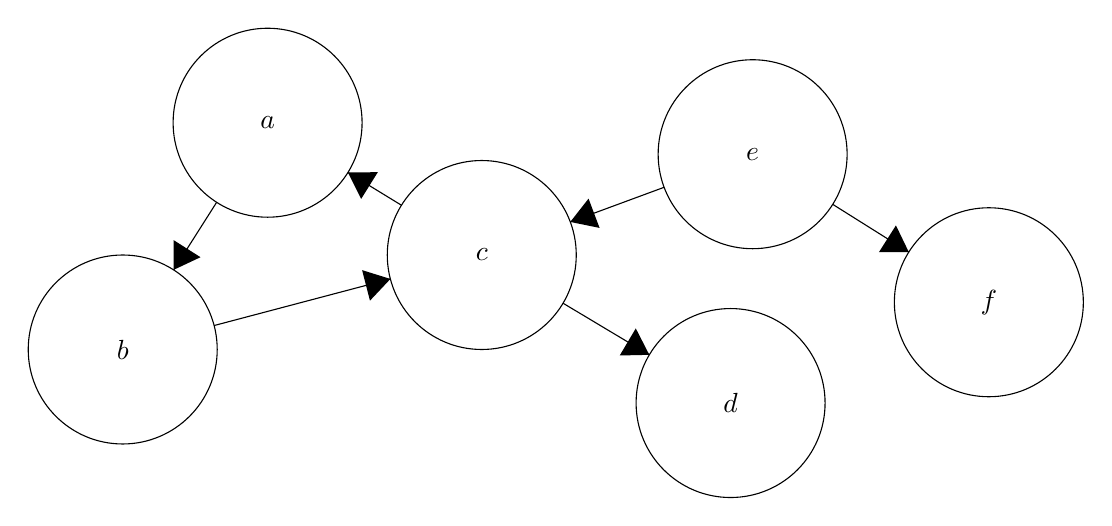
\begin{tikzpicture}[scale=0.4]
\tikzstyle{every node}+=[inner sep=0pt]
\draw [black] (17.4,-25.8) circle (3);
\draw (17.4,-25.8) node {$b$};
\draw [black] (22,-18.6) circle (3);
\draw (22,-18.6) node {$a$};
\draw [black] (28.8,-22.8) circle (3);
\draw (28.8,-22.8) node {$c$};
\draw [black] (36.7,-27.5) circle (3);
\draw (36.7,-27.5) node {$d$};
\draw [black] (37.4,-19.6) circle (3);
\draw (37.4,-19.6) node {$e$};
\draw [black] (44.9,-24.3) circle (3);
\draw (44.9,-24.3) node {$f$};
\draw [black] (20.38,-21.13) -- (19.02,-23.27);
\fill [black] (19.02,-23.27) -- (19.87,-22.87) -- (19.02,-22.33);
\draw [black] (20.3,-25.04) -- (25.9,-23.56);
\fill [black] (25.9,-23.56) -- (25,-23.28) -- (25.25,-24.25);
\draw [black] (26.25,-21.22) -- (24.55,-20.18);
\fill [black] (24.55,-20.18) -- (24.97,-21.02) -- (25.5,-20.17);
\draw [black] (31.38,-24.33) -- (34.12,-25.97);
\fill [black] (34.12,-25.97) -- (33.69,-25.13) -- (33.18,-25.99);
\draw [black] (34.59,-20.65) -- (31.61,-21.75);
\fill [black] (31.61,-21.75) -- (32.54,-21.94) -- (32.19,-21.01);
\draw [black] (39.94,-21.19) -- (42.36,-22.71);
\fill [black] (42.36,-22.71) -- (41.95,-21.86) -- (41.41,-22.71);
\end{tikzpicture}
\end{center}

We mark all of the nodes as unvisited and start at a white node, in our case node a.
\begin{center}
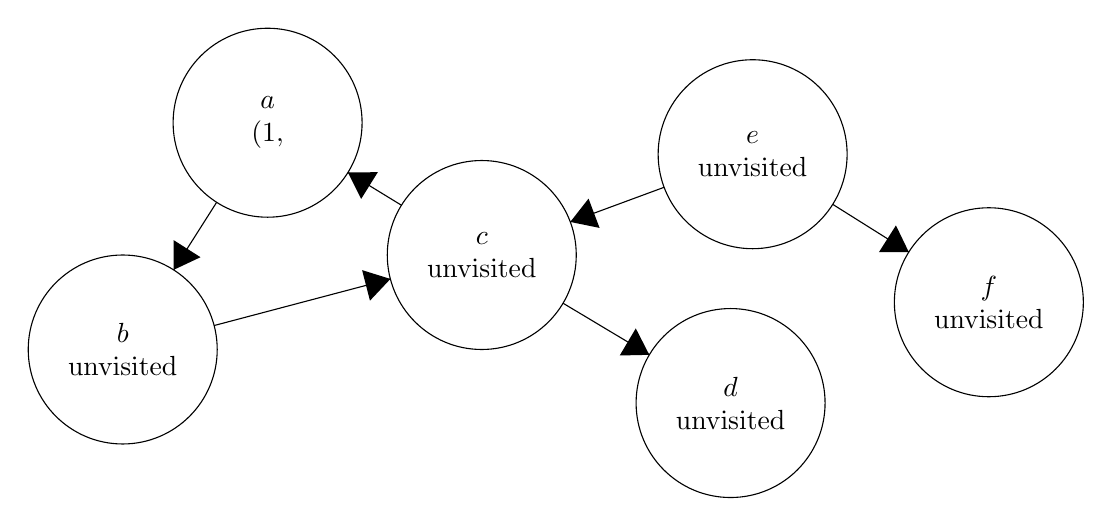
\begin{tikzpicture}[scale=0.4,every text node part/.style={align=center}]
\tikzstyle{every node}+=[inner sep=0pt]
\draw [black] (17.4,-25.8) circle (3);
\draw (17.4,-25.8) node {$b$ \\ unvisited};
\draw [black] (22,-18.6) circle (3);
\draw (22,-18.6) node {$a$ \\ $(1,$};
\draw [black] (28.8,-22.8) circle (3);
\draw (28.8,-22.8) node {$c$ \\ unvisited};
\draw [black] (36.7,-27.5) circle (3);
\draw (36.7,-27.5) node {$d$ \\ unvisited};
\draw [black] (37.4,-19.6) circle (3);
\draw (37.4,-19.6) node {$e$ \\ unvisited};
\draw [black] (44.9,-24.3) circle (3);
\draw (44.9,-24.3) node {$f$ \\ unvisited};
\draw [black] (20.38,-21.13) -- (19.02,-23.27);
\fill [black] (19.02,-23.27) -- (19.87,-22.87) -- (19.02,-22.33);
\draw [black] (20.3,-25.04) -- (25.9,-23.56);
\fill [black] (25.9,-23.56) -- (25,-23.28) -- (25.25,-24.25);
\draw [black] (26.25,-21.22) -- (24.55,-20.18);
\fill [black] (24.55,-20.18) -- (24.97,-21.02) -- (25.5,-20.17);
\draw [black] (31.38,-24.33) -- (34.12,-25.97);
\fill [black] (34.12,-25.97) -- (33.69,-25.13) -- (33.18,-25.99);
\draw [black] (34.59,-20.65) -- (31.61,-21.75);
\fill [black] (31.61,-21.75) -- (32.54,-21.94) -- (32.19,-21.01);
\draw [black] (39.94,-21.19) -- (42.36,-22.71);
\fill [black] (42.36,-22.71) -- (41.95,-21.86) -- (41.41,-22.71);
\end{tikzpicture}
\end{center}

From node $a$ we will visit all of $a$'s children, namely node $b$.

\begin{center}
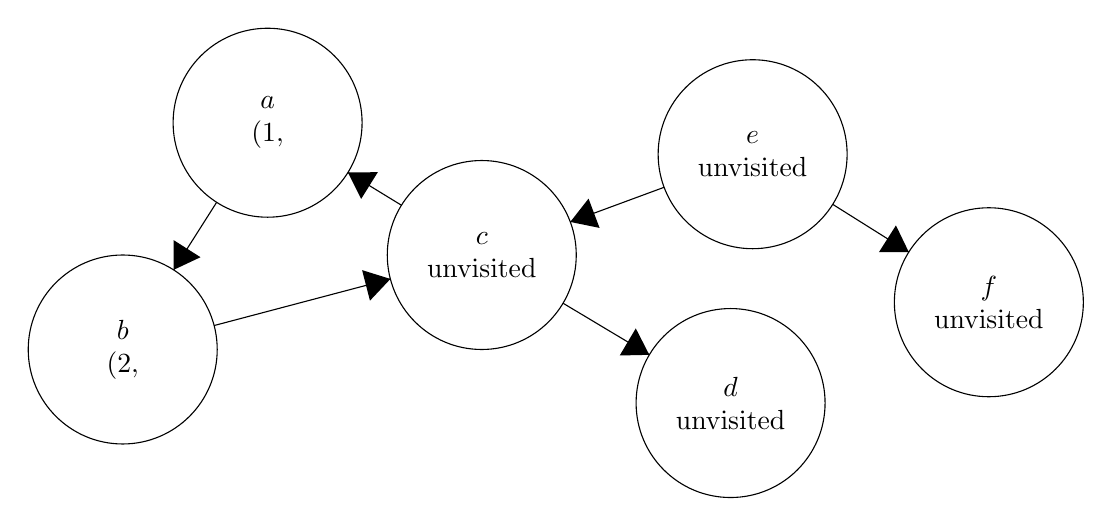
\begin{tikzpicture}[scale=0.4,every text node part/.style={align=center}]
\tikzstyle{every node}+=[inner sep=0pt]
\draw [black] (17.4,-25.8) circle (3);
\draw (17.4,-25.8) node {$b$ \\ $(2,$};
\draw [black] (22,-18.6) circle (3);
\draw (22,-18.6) node {$a$ \\ $(1,$};
\draw [black] (28.8,-22.8) circle (3);
\draw (28.8,-22.8) node {$c$ \\ unvisited};
\draw [black] (36.7,-27.5) circle (3);
\draw (36.7,-27.5) node {$d$ \\ unvisited};
\draw [black] (37.4,-19.6) circle (3);
\draw (37.4,-19.6) node {$e$ \\ unvisited};
\draw [black] (44.9,-24.3) circle (3);
\draw (44.9,-24.3) node {$f$ \\ unvisited};
\draw [black] (20.38,-21.13) -- (19.02,-23.27);
\fill [black] (19.02,-23.27) -- (19.87,-22.87) -- (19.02,-22.33);
\draw [black] (20.3,-25.04) -- (25.9,-23.56);
\fill [black] (25.9,-23.56) -- (25,-23.28) -- (25.25,-24.25);
\draw [black] (26.25,-21.22) -- (24.55,-20.18);
\fill [black] (24.55,-20.18) -- (24.97,-21.02) -- (25.5,-20.17);
\draw [black] (31.38,-24.33) -- (34.12,-25.97);
\fill [black] (34.12,-25.97) -- (33.69,-25.13) -- (33.18,-25.99);
\draw [black] (34.59,-20.65) -- (31.61,-21.75);
\fill [black] (31.61,-21.75) -- (32.54,-21.94) -- (32.19,-21.01);
\draw [black] (39.94,-21.19) -- (42.36,-22.71);
\fill [black] (42.36,-22.71) -- (41.95,-21.86) -- (41.41,-22.71);
\end{tikzpicture}
\end{center}

We now visit b's child, node c.

\begin{center}
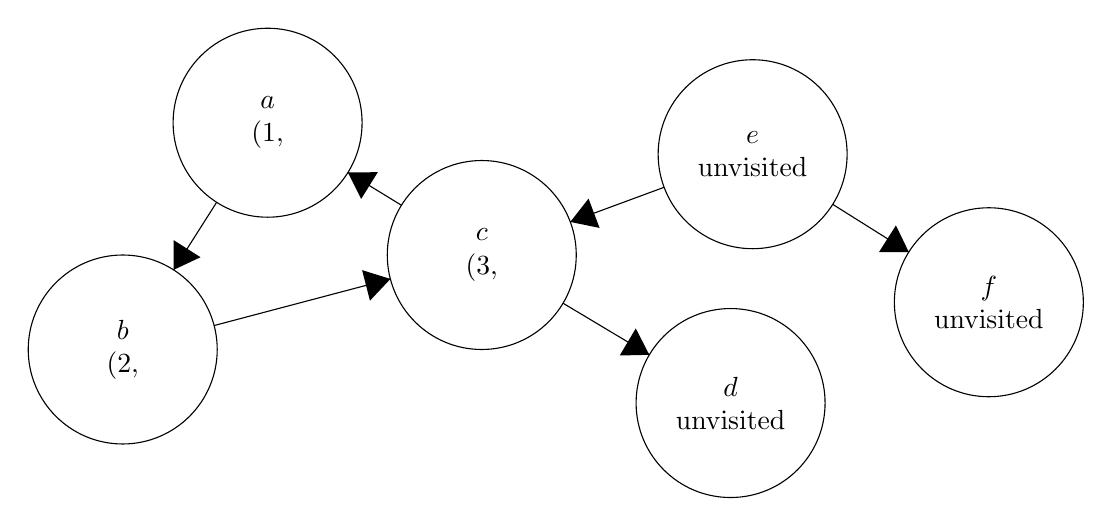
\begin{tikzpicture}[scale=0.4,every text node part/.style={align=center}]
\tikzstyle{every node}+=[inner sep=0pt]
\draw [black] (17.4,-25.8) circle (3);
\draw (17.4,-25.8) node {$b$ \\ $(2,$};
\draw [black] (22,-18.6) circle (3);
\draw (22,-18.6) node {$a$ \\ $(1,$};
\draw [black] (28.8,-22.8) circle (3);
\draw (28.8,-22.8) node {$c$ \\ $(3,$};
\draw [black] (36.7,-27.5) circle (3);
\draw (36.7,-27.5) node {$d$ \\ unvisited};
\draw [black] (37.4,-19.6) circle (3);
\draw (37.4,-19.6) node {$e$ \\ unvisited};
\draw [black] (44.9,-24.3) circle (3);
\draw (44.9,-24.3) node {$f$ \\ unvisited};
\draw [black] (20.38,-21.13) -- (19.02,-23.27);
\fill [black] (19.02,-23.27) -- (19.87,-22.87) -- (19.02,-22.33);
\draw [black] (20.3,-25.04) -- (25.9,-23.56);
\fill [black] (25.9,-23.56) -- (25,-23.28) -- (25.25,-24.25);
\draw [black] (26.25,-21.22) -- (24.55,-20.18);
\fill [black] (24.55,-20.18) -- (24.97,-21.02) -- (25.5,-20.17);
\draw [black] (31.38,-24.33) -- (34.12,-25.97);
\fill [black] (34.12,-25.97) -- (33.69,-25.13) -- (33.18,-25.99);
\draw [black] (34.59,-20.65) -- (31.61,-21.75);
\fill [black] (31.61,-21.75) -- (32.54,-21.94) -- (32.19,-21.01);
\draw [black] (39.94,-21.19) -- (42.36,-22.71);
\fill [black] (42.36,-22.71) -- (41.95,-21.86) -- (41.41,-22.71);
\end{tikzpicture}
\end{center}

Node c has two children that we must visit. When we try to visit node a we find that node a has already been visited (and would be colored gray, as we are in the process of searching a's children), so we do not continue searching down that path. We will next search c's second child, node d.

\begin{center}
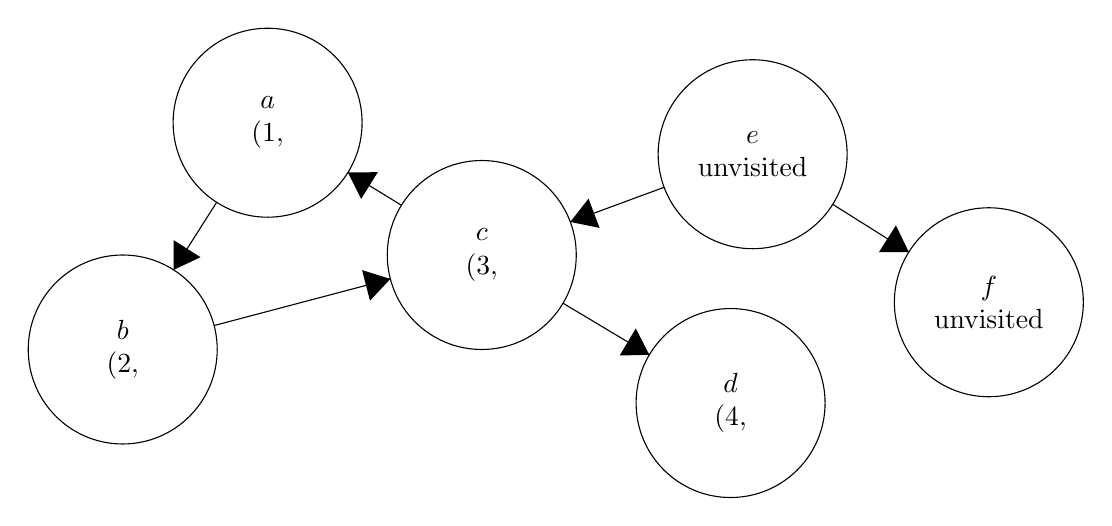
\begin{tikzpicture}[scale=0.4,every text node part/.style={align=center}]
\tikzstyle{every node}+=[inner sep=0pt]
\draw [black] (17.4,-25.8) circle (3);
\draw (17.4,-25.8) node {$b$ \\ $(2,$};
\draw [black] (22,-18.6) circle (3);
\draw (22,-18.6) node {$a$ \\ $(1,$};
\draw [black] (28.8,-22.8) circle (3);
\draw (28.8,-22.8) node {$c$ \\ $(3,$};
\draw [black] (36.7,-27.5) circle (3);
\draw (36.7,-27.5) node {$d$ \\ $(4,$};
\draw [black] (37.4,-19.6) circle (3);
\draw (37.4,-19.6) node {$e$ \\ unvisited};
\draw [black] (44.9,-24.3) circle (3);
\draw (44.9,-24.3) node {$f$ \\ unvisited};
\draw [black] (20.38,-21.13) -- (19.02,-23.27);
\fill [black] (19.02,-23.27) -- (19.87,-22.87) -- (19.02,-22.33);
\draw [black] (20.3,-25.04) -- (25.9,-23.56);
\fill [black] (25.9,-23.56) -- (25,-23.28) -- (25.25,-24.25);
\draw [black] (26.25,-21.22) -- (24.55,-20.18);
\fill [black] (24.55,-20.18) -- (24.97,-21.02) -- (25.5,-20.17);
\draw [black] (31.38,-24.33) -- (34.12,-25.97);
\fill [black] (34.12,-25.97) -- (33.69,-25.13) -- (33.18,-25.99);
\draw [black] (34.59,-20.65) -- (31.61,-21.75);
\fill [black] (31.61,-21.75) -- (32.54,-21.94) -- (32.19,-21.01);
\draw [black] (39.94,-21.19) -- (42.36,-22.71);
\fill [black] (42.36,-22.71) -- (41.95,-21.86) -- (41.41,-22.71);
\end{tikzpicture}
\end{center}

Since node d has no children, we return back to its parent node, c, and continue to go back up the path we took, marking nodes with a finish time when we have searched all of their children.

\begin{center}
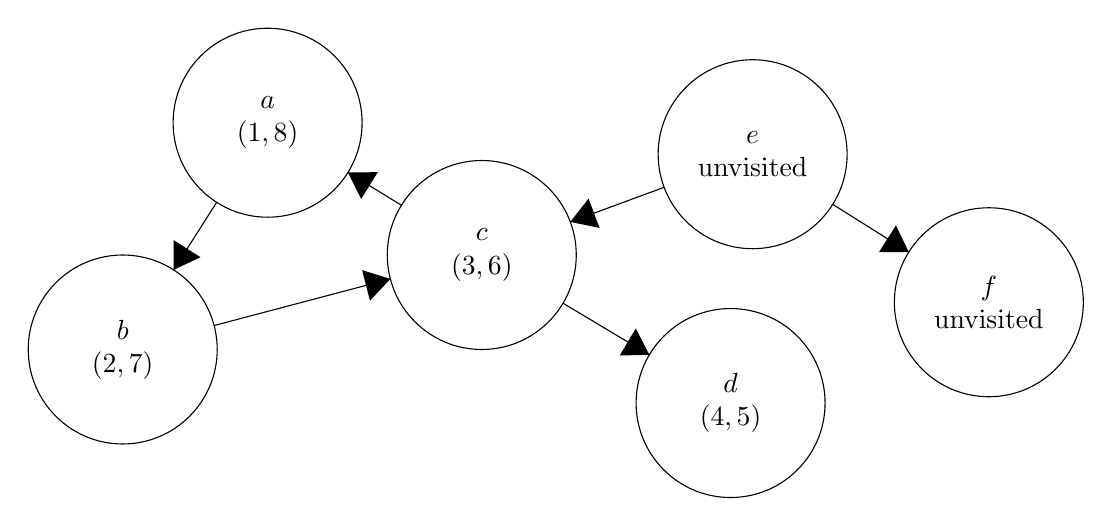
\begin{tikzpicture}[scale=0.4,every text node part/.style={align=center}]
\tikzstyle{every node}+=[inner sep=0pt]
\draw [black] (17.4,-25.8) circle (3);
\draw (17.4,-25.8) node {$b$ \\ $(2,7)$};
\draw [black] (22,-18.6) circle (3);
\draw (22,-18.6) node {$a$ \\ $(1,8)$};
\draw [black] (28.8,-22.8) circle (3);
\draw (28.8,-22.8) node {$c$ \\ $(3,6)$};
\draw [black] (36.7,-27.5) circle (3);
\draw (36.7,-27.5) node {$d$ \\ $(4,5)$};
\draw [black] (37.4,-19.6) circle (3);
\draw (37.4,-19.6) node {$e$ \\ unvisited};
\draw [black] (44.9,-24.3) circle (3);
\draw (44.9,-24.3) node {$f$ \\ unvisited};
\draw [black] (20.38,-21.13) -- (19.02,-23.27);
\fill [black] (19.02,-23.27) -- (19.87,-22.87) -- (19.02,-22.33);
\draw [black] (20.3,-25.04) -- (25.9,-23.56);
\fill [black] (25.9,-23.56) -- (25,-23.28) -- (25.25,-24.25);
\draw [black] (26.25,-21.22) -- (24.55,-20.18);
\fill [black] (24.55,-20.18) -- (24.97,-21.02) -- (25.5,-20.17);
\draw [black] (31.38,-24.33) -- (34.12,-25.97);
\fill [black] (34.12,-25.97) -- (33.69,-25.13) -- (33.18,-25.99);
\draw [black] (34.59,-20.65) -- (31.61,-21.75);
\fill [black] (31.61,-21.75) -- (32.54,-21.94) -- (32.19,-21.01);
\draw [black] (39.94,-21.19) -- (42.36,-22.71);
\fill [black] (42.36,-22.71) -- (41.95,-21.86) -- (41.41,-22.71);
\end{tikzpicture}
\end{center}

Once we reach our first source node a we find that we have searched all of its children, so we look in the graph to see if there are any unvisited nodes remaining. For our example, we start with a new source node e and run DFS to completion.


\begin{center}
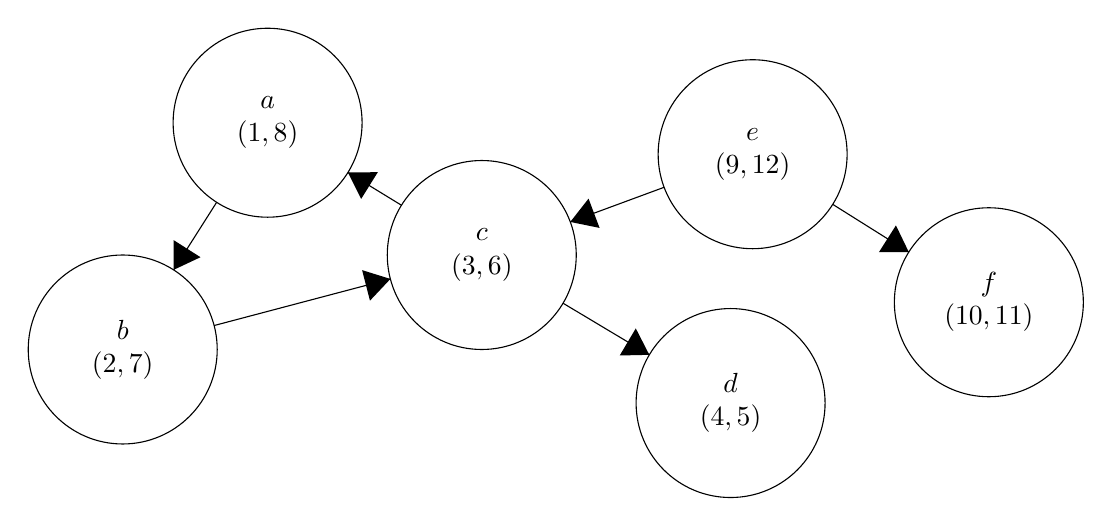
\begin{tikzpicture}[scale=0.4,every text node part/.style={align=center}]
\tikzstyle{every node}+=[inner sep=0pt]
\draw [black] (17.4,-25.8) circle (3);
\draw (17.4,-25.8) node {$b$ \\ $(2,7)$};
\draw [black] (22,-18.6) circle (3);
\draw (22,-18.6) node {$a$ \\ $(1,8)$};
\draw [black] (28.8,-22.8) circle (3);
\draw (28.8,-22.8) node {$c$ \\ $(3,6)$};
\draw [black] (36.7,-27.5) circle (3);
\draw (36.7,-27.5) node {$d$ \\ $(4,5)$};
\draw [black] (37.4,-19.6) circle (3);
\draw (37.4,-19.6) node {$e$ \\ $(9,12)$};
\draw [black] (44.9,-24.3) circle (3);
\draw (44.9,-24.3) node {$f$ \\ $(10,11)$};
\draw [black] (20.38,-21.13) -- (19.02,-23.27);
\fill [black] (19.02,-23.27) -- (19.87,-22.87) -- (19.02,-22.33);
\draw [black] (20.3,-25.04) -- (25.9,-23.56);
\fill [black] (25.9,-23.56) -- (25,-23.28) -- (25.25,-24.25);
\draw [black] (26.25,-21.22) -- (24.55,-20.18);
\fill [black] (24.55,-20.18) -- (24.97,-21.02) -- (25.5,-20.17);
\draw [black] (31.38,-24.33) -- (34.12,-25.97);
\fill [black] (34.12,-25.97) -- (33.69,-25.13) -- (33.18,-25.99);
\draw [black] (34.59,-20.65) -- (31.61,-21.75);
\fill [black] (31.61,-21.75) -- (32.54,-21.94) -- (32.19,-21.01);
\draw [black] (39.94,-21.19) -- (42.36,-22.71);
\fill [black] (42.36,-22.71) -- (41.95,-21.86) -- (41.41,-22.71);
\end{tikzpicture}
\end{center}




























\end{document}


